\chapter{Batch ranking algorithms}
\label{ch:batch_ranking}
In contrary to online ranking algorithms, \textbf{batch ranking algorithms} do not represent player's rating in a single state, but they take in account outcomes of all previous matches in order to establish a leader board.

Although this may seem like a more thorough way to go, processing all previous matches is more computationally complex and may be too computationally difficult for bigger datasets.

\section{Graph-based ranking}
\label{sec:pagerank}
A famous representant of a graph-based ranking system is Google's PageRank introduced by \citet{PagePageRankcitationranking1998} to rank importance of web pages in Google Search Engine. The core idea is that the importance of a page should be based on the number and importance of pages that point to the page. Such idea can be expressed using a recursive formula.

\begin{equation}
r(P) = \sum_{Q \in B_P} \frac{r(Q)}{|Q|},
\label{eq:pagerank}
\end{equation}

\noindent where $r(x)$ is the rating of page $x$, $Q \in B_P$ is the set of all pages $Q$ pointing to page $P$ and $|Q|$ is the number of pages Q is pointing to. This shows that the more pages a page points to, the more the page lowers its effect on the importance of these pages and therefore the importance of a page can be viewed as number of \textit{votes} the page can \textit{vote} in favor of other pages.

All of the pages indexed by Google create a directed graph of pages pointing to each other. Since the PageRank formula \eqref{eq:pagerank} is recursive, the nodes of the graph are initialized at the same value and then the PageRank of each node is iteratively updated until the value of PageRank converges. This can be expressed as follows.

\begin{equation*}
r_{i+1}(P) = \sum_{Q \in B_P} \frac{r_i(Q)}{|Q|} ,\quad i = 0, 1, 2, \dots,
\end{equation*}

\noindent where $r_{i+1}(P)$ is the rating of page P in iteration $i+1$, while $r_i(Q)$ is the rating of page Q in iteration $i$.

\subsection{Adapting PageRank to soccer}
As \citet{LazovaPageRankApproachRanking2015} explain, in order to adapt PageRank algorithm to soccer games, nodes of the graph represent teams instead of pages. An edge exists between all nodes that represent teams that have played a match against each other. Note that in difference to the PageRank's original graph, teams always have an edge in both directions. The values of the edges are calculated by a function that can take into account any information about the teams' relations (win/lose ratio, goals scored, number of draws, \dots).

Let matrix $A$ be the adjacency matrix of said graph. As \citet{GOVANRANKINGNATIONALFOOTBALL} explain, in order to ensure the convergence of PageRank algorithm, a matrix $Q$ is derived from A as follows.

\begin{align}
\label{eq:a_to_q}
Q_{i,j} = (1-d)\cdot \frac{A_{i,j}}{\sum_{k=1}^{N} A_{i,k}} + \frac{d}{N}
\end{align}

\noindent with $A_{i,j}$ representing $i$-th row and $j$-th column of the matrix A and $N$ representing number of teams.

Similarily to the original PageRank algorithm, the PageRank value of each team is calculated by the iterative process. After the ratings have converged, teams ratings will be represented by a value from the interval $(0, 1)$ with greater values expressing the team is stronger.

\examplespace
\begin{example}
To obtain a better understanding of PageRank, let's rank four teams A, B, C and D that have played following matches:\\[0.5em]
\begin{tabular}{l c r} 
A & 3:1 & B \\
A & 2:1 & C \\
B & 1:1 & C \\
B & 2:0 & D \\
\end{tabular}\\[0.5em]
meaning that A has won three matches against B and lost one, B has defeated C in two matches and have not lost a single match, etc.
For simplicity, we will disregard number of goals scored.

For a better visualization of the match-ups, a bidirectional graph can be constructed. Note that the weight of the edges denotes how many \textit{votes} does a team give in favor of the other team, therefore for teams A and B, the weight of edge from A to B is 1 and 3 for the edge from B to A.

\vspace{1em}
\begin{figure}[H]
\centering
\begin{tikzpicture}
  \SetGraphUnit{3}
  \Vertex{B}
  \NOWE(B){A}
  \SOWE(B){C}
  \EA(B){D}
  \Edge[label = 1](A)(B)
  \Edge[label = 1](B)(C)
  \Edge[label = 1](A)(C)
  \Edge[label = 0](B)(D)
  \tikzset{EdgeStyle/.append style = {bend left = 50}}
  \Edge[label = 2](C)(A)
  \tikzset{EdgeStyle/.append style = {bend right = 50}}
  \Edge[label = 2](D)(B)
  \Edge[label = 3](B)(A)  
  \Edge[label = 1](C)(B)
\end{tikzpicture}
\end{figure}

A weighting function has to be applied to achieve proper values of the edges. For simplicity of the example, following function is applied.

\begin{equation*}
f_{i,j} = \frac{w_{i,j}}{g_{i,j}},
\end{equation*}

\noindent where $f_{i,j}$ is the calculated weight between nodes $i$ and $j$, $w_{i,j}$ is number of matches won by $i$ against $j$ and $g_{i,j}$ is number of total games played between $i$ and $j$. After applying such function on every edge, the graph looks as follows. Also, this introduces the \textit{damping factor} $d$, which adds some randomness to the procedure. This ensures that the iterative procedure will eventually converge. Also, the damping factor is somewhat intuitive, because it adds a small winning probability for teams that have never played against each other. The damping factor is user-defined and the authors of PageRank suggest using conservative value of 0.15.

Then, the PageRanks are assigned initial values and the algorithm iterates until the values converge. In every iteration, following equation is executed, leading to the change in PageRank values.

\begin{equation*}
\pi_{t+1}^T = \pi_t^TQ,\quad t= 0, 1, 2, \dots,
\end{equation*}

with $t$ representing current iteration and $\pi_t$ vector of PageRanks in current iteration. Note that $\pi_0$ can be chosen either randomly or homogeneously.

\vspace{1em}
\begin{figure}[H]
\centering
\begin{tikzpicture}
  \SetGraphUnit{3}
  \Vertex{B}
  \NOWE(B){A}
  \SOWE(B){C}
  \EA(B){D}
  \Edge[label = $\frac{1}{4}$](A)(B)
  \Edge[label = $\frac{1}{2}$](B)(C)
  \Edge[label = $\frac{1}{3}$](A)(C)
  \Edge[label = 0](B)(D)
  \tikzset{EdgeStyle/.append style = {bend left = 50}}
  \Edge[label = $\frac{2}{3}$](C)(A)
  \tikzset{EdgeStyle/.append style = {bend right = 50}}
  \Edge[label = 1](D)(B)
  \Edge[label = $\frac{3}{4}$](B)(A)  
  \Edge[label = $\frac{1}{2}$](C)(B)
\end{tikzpicture}
\end{figure}

\noindent which corresponds to following adjacency matrix.

\[
\renewcommand\arraystretch{1.5}
A = 
\begin{bmatrix}
0 & \frac{1}{4} & \frac{1}{3} & 0 \\
\frac{3}{4} & 0 & \frac{1}{2} & 0 \\
\frac{2}{3} & \frac{1}{2} & 0 & 0 \\
0 & 1 & 0 &0
\end{bmatrix}
\]  

In the next step, the adjacency matrix A is converted to matrix Q using formula \eqref{eq:a_to_q}. For the sake of easier calculation, we have chosen the damping factor $d = \frac{1}{5}$ for this example, hence the matrix Q:

\[
\renewcommand\arraystretch{1.5}
Q = 
\begin{bmatrix}
\frac{1}{20} & \frac{55}{140} & \frac{71}{140} & \frac{1}{20} \\
\frac{53}{100} & \frac{1}{20} & \frac{37}{100} & \frac{1}{20} \\
\frac{71}{140} & \frac{55}{140} & \frac{1}{20} & \frac{1}{20} \\
\frac{1}{20} & \frac{17}{20} & \frac{1}{20} & \frac{1}{20}
\end{bmatrix}
\]

Now, a vector of teams' PageRank values $\pi_0^T$ is created. This vector is then iteratively multiplied with the matrix Q until the values converge. We can conservatively initialize the PageRank values to the same value for every team:

\begin{equation*}
\pi_0^T = 
\begin{bmatrix}
\frac{1}{4} & \frac{1}{4} & \frac{1}{4} & \frac{1}{4}
\end{bmatrix}
\end{equation*}

Finally, the iterative procedure starts. For this example, one iteration of the procedure is calculated:

\begin{equation*}
\pi_{t+1}^T = \pi_t^TQ,\quad t= 0, 1, 2, \dots
\end{equation*}

Therefore, the first iteration of our example is calculated as follows.

\begin{align*}
\pi_1^T &= 
\begin{bmatrix}
\frac{1}{4} & \frac{1}{4} & \frac{1}{4} & \frac{1}{4}
\end{bmatrix} 
\cdot
\begin{bmatrix}[1.5]
\frac{1}{20} & \frac{55}{140} & \frac{71}{140} & \frac{1}{20} \\
\frac{53}{100} & \frac{1}{20} & \frac{37}{100} & \frac{1}{20} \\
\frac{71}{140} & \frac{55}{140} & \frac{1}{20} & \frac{1}{20} \\
\frac{1}{20} & \frac{17}{20} & \frac{1}{20} & \frac{1}{20}
\end{bmatrix} \\[1em]
&= 
\begin{bmatrix}
\frac{859}{3200} & \frac{59}{115} & \frac{171}{700} & \frac{1}{20}
\end{bmatrix}
\end{align*}

The vector $\pi_1^T$ holds the teams' PageRanks after first iteration. In order to calculate next iteration's result, the same matrix Q is multiplied with $\pi_1^T$ obtained in the first iteration.

After the algorithm converges, the values in $\pi$ are teams' final PageRanks. Higher PageRank of a team means that the team is considered to be better. Therefore, in this example after the first iteration, player B is considered to be the best one, A the second, C the third and D is the worst.
\end{example}

\subsection{Cons of PageRank}
While other ranking algorithms usually perceive team as a set of individuals, PageRank perceives a team as a blackbox. This leads to lack of knowledge about individual players, which makes for the disability of examining players' skill individually. Also, changes in team's structure are not projected to the team's PageRank rating, which is a solid property for building leader boards, but it causes difficulties in matching teams with equally strong opponents.

\subsection{Applying graph-based ranking on real data}
Using the PageRank algorithm adapted for soccer games, an empty oriented graph with nodes representing teams is created and fit with appropriate data. After the graph is created, the edges are assigned weights using functions listed below. 

\vspace{1em}
\begin{tabular}{l}
$f_{i,j} = \frac{\ell_{i,j}}{g_{i,j}}\cdot \frac{1}{G-g_{i,j}+1}$\\[1em]
$f_{i,j} = \frac{\ell_{i,j}}{g_{i,j}}$\\[1em]
$f_{i,j} = \frac{\ell_{i,j}}{g_{i,j}} + \frac{c_{i,j}}{c_{i,j}+s_{i,j}}$\\[1em]
$f_{i,j} = \ell_{i,j}$\\[1em]
$f_{i,j} = \frac{c_{i,j}}{s_{i,j}}$\\[1em]
$f_{i,j} = \frac{\ell_{i,j}}{w_{i,j}}$\\[1em]
$f_{i,j} = \frac{\ell_{i,j}}{g_{i,j}}+0.5\cdot \frac{d_{i,j}}{g_{i,j}}$\\[1em]
$f_{i,j} = \frac{c_{i,j}}{c_{i,j}+s_{i,j}}$\\[1em]
$f_{i,j} = \frac{c_{i,j}}{g_{i,j}}$\\[1em]
$f_{i,j} = c_{i,j}$
\end{tabular}
\vspace{1em}

\noindent where\\

\vspace{-1.2em}
\begin{table}[H]
\begin{tabular}{rl}
$f_{i,j}$\quad &is the weight of edge from $i$ to $j$,\\
$g_{i,j}$\quad &is the number of games played between $i$ and $j$,\\
$\ell_{i,j}$\quad &is the number of games $i$ lost against $j$,\\
$w_{i,j}$\quad &is the number of games $i$ won against $j$,\\
$d_{i,j}$\quad &is the number of games drawn between $i$ and $j$,\\
$c_{i,j}$\quad &is the number of goals $j$ has scored in all matches against $i$,\\
$s_{i,j}$\quad &is the number of goals $i$ has scored in all matches against $j$,\\
$G$\quad &is the maximum number of games played between any two teams
\end{tabular}
\end{table}
\vspace{-1em}

After determining the weights of the graph, the graph is represented as a matrix and the PageRank iterative procedure calculates appropriate PageRank of every function used. The goal is to detect such function that will be most successful in predicting outcomes of given matches. To calculate the belief in a team's victory, Bradley-Terry model with given team's PageRank $\pi_A$ as his score, hence \eqref{eq:pagerank_bradley_terry}.

\begin{equation}
\label{eq:pagerank_bradley_terry}
P(A > B) = \frac{\pi_A}{\pi_A + \pi_B}
\end{equation}

Following such principle for every PageRank's weighting function, results as shown in \autoref{table:pagerank_results} were obtained.

\vspace{1em}
\begin{table}[H]
\caption{Results of different weighting functions used with the extended PageRank algorithm}
\label{table:pagerank_results}
\begin{tabular}{| l | r | r |}
\hline
\textbf{Function} & \textbf{Matches predicted} & \textbf{Log-likelihood loss} \\ \hline
$\frac{\ell_{i,j}}{g_{i,j}}\cdot \frac{1}{G-g_{i,j}+1}$ &  36.55 & 0.695 \\ \hline
$\frac{\ell_{i,j}}{g_{i,j}}$ &  38.34 & 0.679 \\ \hline
$\frac{\ell_{i,j}}{g_{i,j}} + \frac{c_{i,j}}{c_{i,j}+s_{i,j}}$ &  36.06 & 0.684 \\ \hline
$\ell_{i,j}$ &  34.82 & 0.722 \\ \hline
$\frac{c_{i,j}}{s_{i,j}}$ &  37.14 & 0.679 \\ \hline
$\frac{\ell_{i,j}}{w_{i,j}}$ &  37.90 & 0.713 \\ \hline
$\frac{\ell_{i,j}}{g_{i,j}}+0.5\cdot \frac{d_{i,j}}{g_{i,j}}$ &  36.46 & 0.683 \\ \hline
$\frac{c_{i,j}}{c_{i,j}+s_{i,j}}$ &  34.79 & 0.690 \\ \hline
$\frac{c_{i,j}}{g_{i,j}}$ &  34.77 & 0.694 \\ \hline
$c_{i,j}$ & 31.49 & 0.750 \\ \hline
\end{tabular}
\end{table}

\section{Supervised Learning approach to match prediction}
Supervised Learning is a machine learning task of approximating a function based on known input-output pairs. Such input-output pairs consist of an input vector, which represents the argument to the approximated function, and an output vector, which holds the output of the function. The Supervised Learning algorithm analyzes the training data in order to create a function that can then be used to calculate outputs. In other words, Supervised Learning is an algorithm solving a regression task.

Numerous approaches to Supervised Learning exist, from simpler ones like Linear or Logistic Regression, to more complicated ones like Support Vector Machines or Neural Networks. For the task of predicting outcomes of soccer matches, we have decided to use Multilayer Perceptron, which is a feedforward artificial Neural Network.

The Multilayer Perceptron has been chosen as the Supervised Learning algorithm due to recent popularity of Neural Networks, as well as their capability of approximating any function, if the right network structure is used. This is shown has been shown by \citet{HornikApproximationCapabilitiesMultilayer1991} and is known as the Universal approximation theorem.

\subsection{Perceptron}
Simple Perceptron introduced by \citet{RosenblattPerceptronProbabilisticModel1958} is an algorithm for Supervised Learning that is able to classify linearly separable set of data. It often represents a single neuron in a Neural Network and it can be visualized as shown in figure \ref{fig:perceptron_tikz}.

\vspace{1em}
\begin{figure}[H]
\caption{Perceptron}
\label{fig:perceptron_tikz}
\centering
\begin{tikzpicture}
  % Vertices
  \node[vertex] (x1) at (0,3)  {$x_1$};
  \node[weights] (w1) at (1.5,3) {$w_1$};
  \node[vertex] (x2) at (0,2)  {$x_2$};
  \node[weights] (w2) at (1.5,2) {$w_2$};
  \node[vertex] (xn) at (0, 0) {$x_n$};
  \node[weights] (wn) at (1.5,0) {$w_n$};
  \node[vertex] (f) at (4, 1.5) {$\mathlarger{\sum}$};
  \node[vertex] (b) at (4, 0) {$\theta$};
  \node[vertex, text width=2.5em] (step) at (6, 1.5) {};
  \node[vertex] (y) at (8, 1.5) {$y$};
  
  % Comments
  \node[note] (x_note) at (0, -0.8) {Inputs};
  \node[note] (w_note) at (1.5, -0.8) {Weights};
  \node[note] (b_note) at (4, -0.7) {Bias};  
  \node[note, text width=4em, text centered] (activation_note) at (6, 0.3) {Activation function};  
  \node[note] (y_note) at (8, 0.8) {Output};  
  
  % Dots between x_2 and x_n
  \node[below of=x2] (dots) {$\vdots$};
  \node[below of=w2] (dots) {$\vdots$};

  % Edges
  \draw (x1) edge [->, draw=black!50] (w1);
  \draw (x2) edge [->, draw=black!50] (w2);
  \draw (xn) edge [->, draw=black!50] (wn);
  \draw (w1) edge [->, draw=black!50] (f);
  \draw (w2) edge [->, draw=black!50] (f);
  \draw (wn) edge [->, draw=black!50] (f);
  \draw (step) edge [->, draw=black!50] (y);
  \draw (f) edge [->, draw=black!50] (step);
  \draw[dashed] (b) edge [->, draw=black!50] (f);
  
  % Step function
  \draw[ultra thick] (5.7,1.3) -- (6,1.3) -- (6,1.8) -- (6.3,1.8);
  \draw (6,1.1) -- (6,1.9);
  \draw (5.6,1.5) -- (6.4,1.5);
\end{tikzpicture}
\end{figure}

In the figure, $(x_1, x_2, \cdots, x_n)$ represents the vector of inputs with appropriate weights $(w_1, w_2, \cdots, w_3)$. Another important feature is the $\theta$, which represents threshold of the Perceptron. This can be expressed mathematically as

\begin{align*}
\sum_{i=1}^{n}{x_i\cdot w_i} \geq \theta.
\end{align*}

The threshold can also be perceived as an additional input with weight of 1, creating vectors of inputs and appropriate weights $(-\theta, x_1, x_2, \cdots, x_n)$ and $(1, w_1, w_2, \cdots, w_n)$, respectively. The product of such two vectors $\xi$ is called \textit{potential} and is passed as an argument to an activation function, which outputs the actual result of the Perceptron. Therefore, the output of the Perceptron can be expressed as

\begin{align*}
y = f\left(\sum_{i=0}^{n}{x_i\cdot w_i}\right),
\end{align*}

\noindent where $f(\cdot)$ is the activation function.

There are numerous activation function that can be used, from which an example of few is provided.
\begin{itemize}
\item Binary step: $$y = \begin{cases}1 & if \sum\limits_{i=0}^{n}{x_i\cdot w_i} \geq 0 \\ 0 & if \sum\limits_{i=0}^{n}{x_i\cdot w_i} < 0,\end{cases}$$
\item Logistic: $$f(\xi) = \frac{1}{1+e^{-\xi}}, \qquad \xi = \sum_{i=0}^{n}{x_i\cdot w_i},$$
\item Gaussian: $$f(\xi) = e^{-\xi^2}, \qquad \xi = \sum_{i=0}^{n}{x_i\cdot w_i}.$$
\end{itemize}

After the output si known, the Perceptron compares the actual output with the presented output and adjusts the weights accordingly. Input samples are presented to the algorithm until it converges and separates the data. Note that as \citet{NovikoffConvergenceProofsPerceptrons1962} stated, the convergence of the Perceptron is certain.

Then the Perceptron is considered trained and new inputs can be presented to predict their output based on the separation of the data.

\subsection{Multilayer Perceptron}
\label{sec:multilayer_perceptron}
Unfortunately, the Perceptron's ability in separating data is limited. It often happens that the separation is not sufficient and multiple Perceptrons have to be used in multiple layers in order to achieve more precise data separation, creating a Multilayer Perceptron of $n \geq 2$ layers. In such $n$ layers, there is always one input layer with $m = |x|$ neurons, every neuron accepting one element of the input vector $x$. The input layers is fully connected to $n-2$ hidden layers with no strict restriction on number of neurons. Also, every $i$-th hidden layer is fully connected to $(i+1)$-th layer. Finally, the last layer is the output layer, presenting outputs of given inputs, also fully connected to the last hidden layer. This can be visualized as follows.

\vspace{1em}
\begin{figure}[H]
\caption{Multilayer Perceptron}
\centering
\begin{tikzpicture}[shorten >=1pt,->,draw=black!50, node distance=\layersep]
    \tikzstyle{every pin edge}=[<-,shorten <=1pt]
    \tikzstyle{annot} = [text width=4em, text centered]

    % Draw the input layer nodes
    \foreach \name / \y in {1,...,2}
    % This is the same as writing \foreach \name / \y in {1/1,2/2,3/3,4/4}
        \node[vertex] (I-\name) at (0,-\y) {$x_\y$};
    \node[vertex] (I-3) at (0,-4) {$x_n$};

    % Draw the hidden layer nodes
    \foreach \name / \y in {1,...,5}
        \path[yshift=0.5cm]
            node[vertex, text width=1.2em] (H-\name) at (\layersep,-\y cm) {};

    % Draw the output layer node
    \node[vertex, pin={[pin edge={->}]right:Output}, right of=H-3] (O) {$y$};

    % Connect every node in the input layer with every node in the
    % hidden layer.
    \foreach \source in {1,...,3}
        \foreach \dest in {1,...,5}
            \path (I-\source) edge (H-\dest);

    % Connect every node in the hidden layer with the output layer
    \foreach \source in {1,...,5}
        \path (H-\source) edge (O);

    % Annotate the layers
    \node[annot,above of=H-1, node distance=1cm] (hl) {Hidden layer};
    \node[annot,left of=hl] {Input layer};
    \node[annot,right of=hl] {Output layer};
    
     \node[] at(0,-3) (dots) {$\vdots$};
\end{tikzpicture}
\end{figure}

As the figure implies, every edge represents a weight and every node a neuron with appropriate value. The neuron's value is calculated similarly as in the Perceptron as a product of inputs and weights. Note that every layer has its own threshold value. 
After the output is determined, an error with respect to the presented output is calculated and the weights are modified accordingly. One of the algorithms used to modify the weights accordingly to the error is the backpropagation algorithm \citep{RumelhartNeurocomputingFoundationsResearch1988}. After the weights are modified, the algorithm iteratively presents inputs to the network until the error of the network $E$ is smaller than a predefined value. The error $E$ is calculated as

\begin{align*}
E = \frac{1}{2}\sum_{p}\sum_{o}(y_{o,p} - d_{o,p})^2,
\end{align*}

\noindent where $p$ is the set of all patterns, $o$ is the vector of output neurons and $y_{o,p}$ and $d_{o,p}$ are the calculated and desired outputs of input $p$ on output neuron $o$, respectively. This is called the mean squared error and is merely one of the functions that can be used to calculate the error.

After the network converges, new inputs can be presented to obtain a regression of outputs.

\subsection{Applying MLP on soccer data}
The Multilayer Perceptron can be applied on soccer data by presenting known matches with their outcomes to the network and obtaining predictions of unknown matches.

\subsubsection{Data preprocessing}
In order to achieve more accurate predictions, preprocessing of the data is required. The input data are presented as a vector of all players, while $1$ represents a player that belongs to the home team in given match, $-1$ a player that played in the away team and $0$ if the player have not played in the particular match. The outputs are based on goal difference in the particular match between $i$-th and $j$-th team and are calculated as

\begin{align*}
y = \frac{s_i}{s_i + s_j},
\end{align*}

\noindent with $s$ representing the goals scored by given team.

\examplespace
\begin{example}
To provide a better understanding of how soccer data are presented to the network, consider a match between team $i$ of players $A, C$ and team $j$ of players $D$ and $F$. Also, consider that team $i$ has won the game by scoring 3 goals in contrary to team $j$, which scored $1$ goal, and that players $B$ and $E$ have not taken place in the match. Then the input vector would be presented to the network as

\begin{align*}
x = \begin{bmatrix}
1 & 0 & 1 & -1 & 0 & -1
\end{bmatrix}
\end{align*}

\noindent where $x_1$ would be presented to the first input neuron, $x_2$ to the second, \dots

The output vector would be

\begin{align*}
y = \begin{bmatrix}
\frac{3}{4}
\end{bmatrix}.
\end{align*}
\end{example}

\subsubsection{Network structure}
In the process of predicting matches, the network structure is significantly influential. There are many parameters that can be set differently and every settings produces a slightly different results. Here are the parameters we have used for outcome predictions:

\begin{itemize}
\item \textbf{Activation function} decides what the output value of a neuron is. Since the soccer predictions represent probabilities of a team's victory, it is desired for the activation function's output to be from the interval $[0, 1]$. Therefore, we have used the softmax activation function, which is a generalization of the logistic function frequently used throughout this thesis. On the hidden layers, linear function is used, making the output reflect the input.

\item \textbf{Loss function} calculates the error of the network. In the description of MLP, mean squared error was mentioned as a loss function. This is, however, optional and different functions can be used. For soccer games, categorical cross entropy function was used, as it produces lower errors than mean squared error function if the matches are closer to its presented category.

\item \textbf{Optimizer} is an algorithm that helps the network find the appropriate weights faster. For purpose of predicting soccer games, the RMSProp algorithm is used, which modifies the learning rate (i.e. how significantly are the weights updated) with respect to the function's gradient. In contrary to AdaGrad algorithm, which is the algorithm RMSProp is based upon, it gives smaller significance to gradients calculated in previous iterations.

\item \textbf{Number of epochs} determines how many iterations of the whole dataset should be used to train the network. For the match predictions, multiple choices of number of epochs were used, although greater numbers led to worse final predictions. 

\item \textbf{Batch size} establishes how many inputs should be processed before adjusting the weights based on the error. Note that higher numbers generally lead to smaller significance of outliers while lower numbers lead to more frequent update of the weights and therefore bigger chance of finding appropriate result sooner. Again, multiple choices were tested on the network, usually achieving better results with lower values.

\item \textbf{Number of layers and neurons} decides how many hidden layers should be used with how many neurons. This is most certainly a tricky attribute and no direct instruction on how many layers to use when exists. Multiple options were tried, leading to a conclusion that one hidden layer with ten neurons produces sufficient results. Note that with increasing number of layers and neurons, the computational complexity increases excessively.
\end{itemize}

\subsection{Results}
Using Multilayer Perceptron for predicting outcomes of matches, solid prediction ability of \textasciitilde 45\% was achieved. However, the result can vary a lot by current structure of the network and parameter settings. 

It is also important to note that the error on training data has decreased throughout epochs, while error on validation data has increased as shown in \ref{fig:overfitting}. This is an indicator of overfitting \citep{CaruanaOverfittingNeuralNets2000}.

\begin{figure}[H]
\caption{Comparison of training and validation loss}
\label{fig:overfitting}
\centering
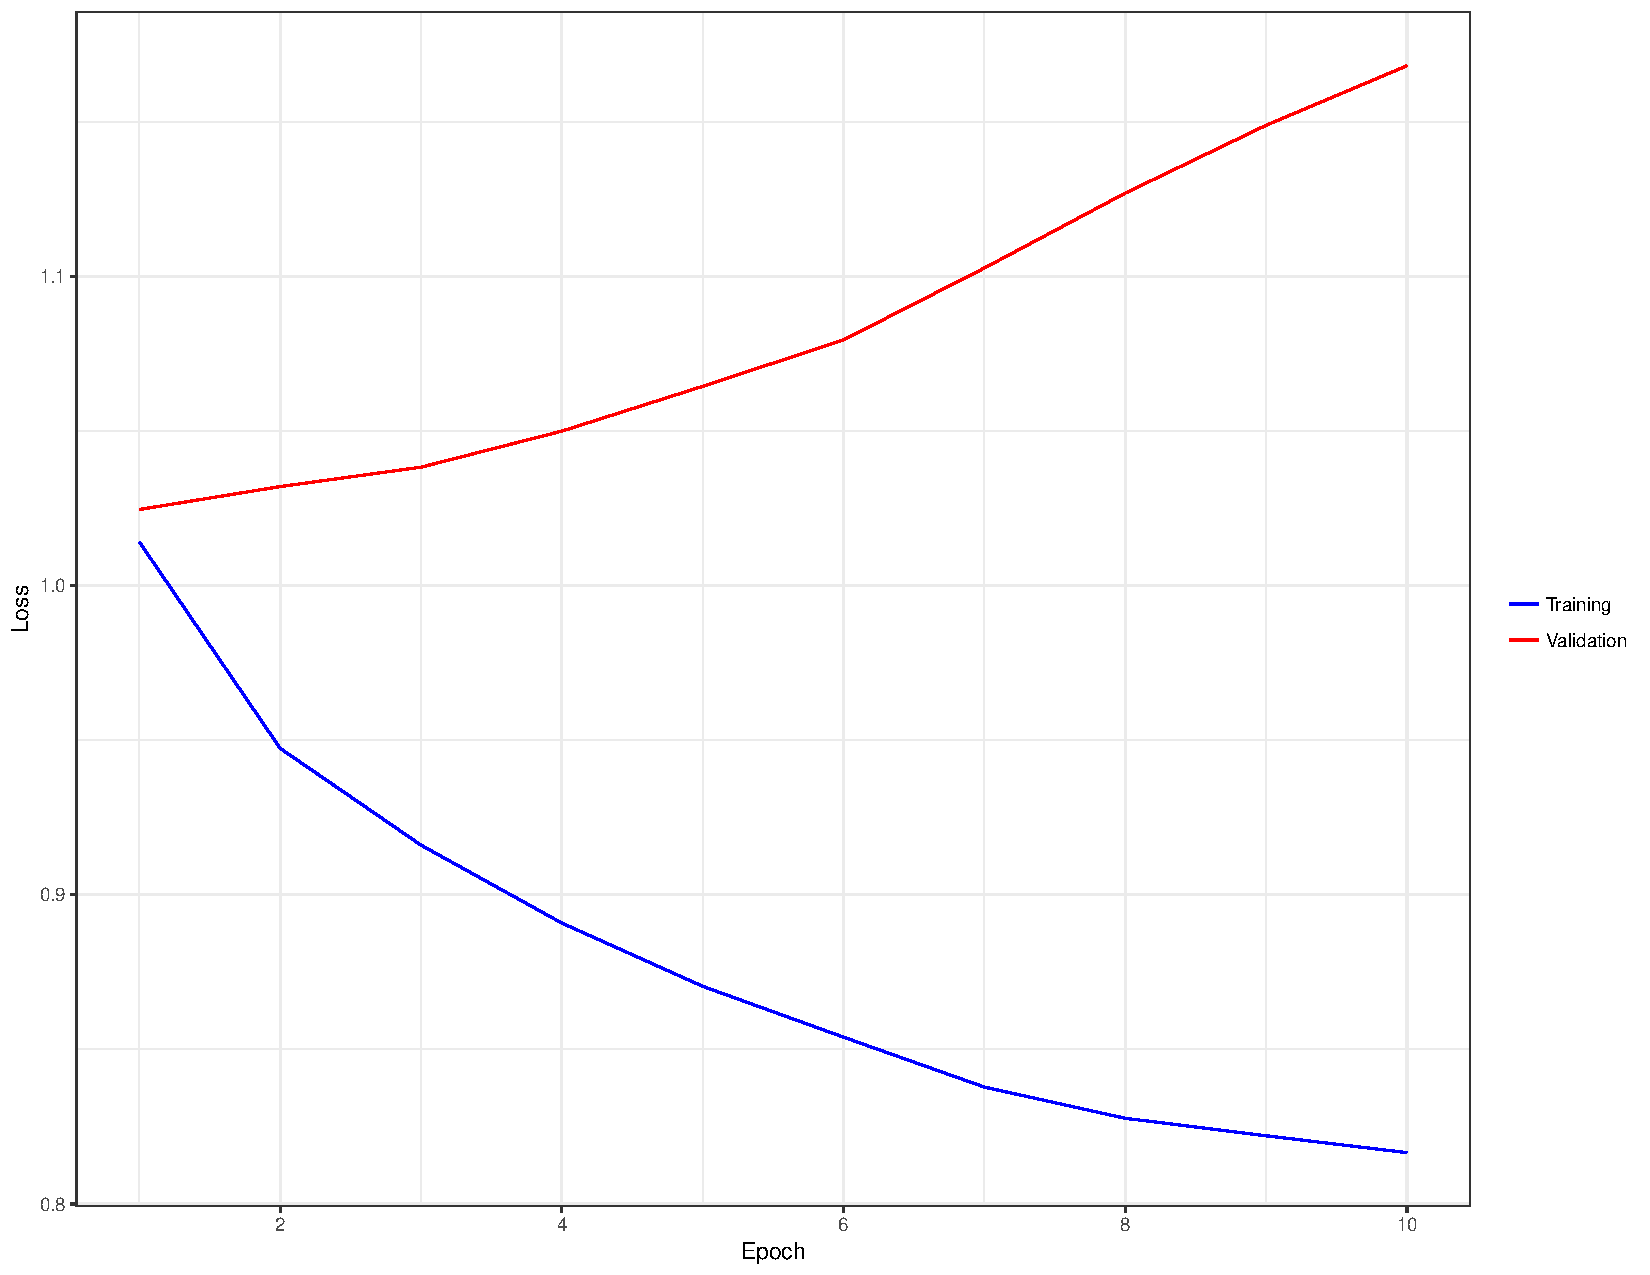
\includegraphics[width=0.8\textwidth]{figs/overfitting}
\end{figure}

Overfitting is believed to happen, among other cases, when the number of trainable parameters is too high compared to the number of data points. In the case of predicting soccer matches, we have 10787 input neurons, each neuron representing a player's relation to given match, and 21373 data points, each representing a match. That is, perhaps, insufficient number of matches given the number of players and therefore, the overfitting problem could be solved by introducing more matches to the network. However, since more data is not available, a method called dropout \citep{SrivastavaDropoutSimpleWay2014} helping to overcome ovefitting has been introduced to the hidden layer. Dropout determines the probability of ignoring a certain neuron and therefore precludes overfitting. By using a dropout probability of 0.4, much better results were achieved as the prediction ability increased to \textasciitilde 49\% and the validation loss was somewhat constant throughout the epochs.

\begin{figure}[H]
\caption{Comparison of training and validation loss with dropout}
\centering
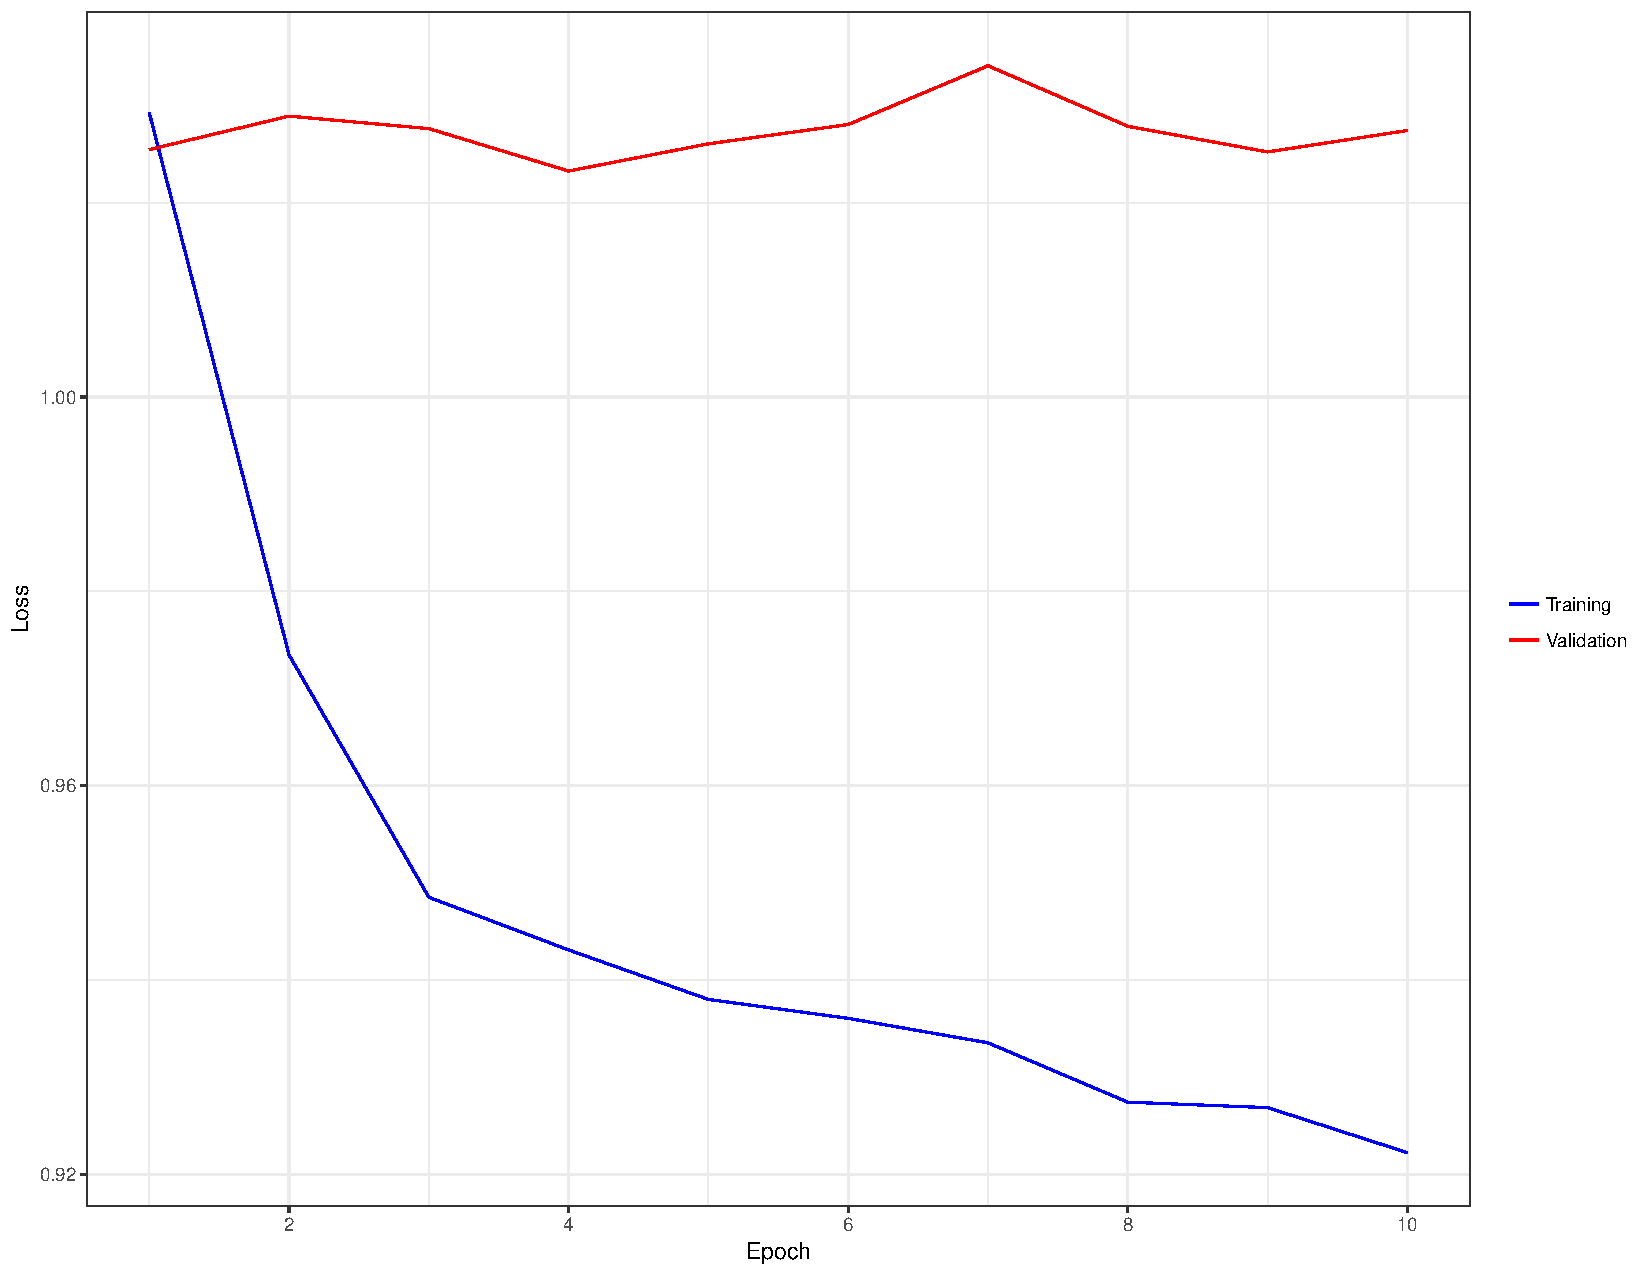
\includegraphics[width=0.8\textwidth]{figs/overfitting_dropout}
\end{figure}

Although Multilayer Perceptron is an easy and effective algorithm to predict outcomes, it does not determine a rating to be assigned to players and therefore does not provide the same possibilities as other ranking algorithms do, e.g. building a leader board.

\section{Maximum likelihood method}
Another approach to ranking teams is the maximum likelihood method. As long as draws are ignored, a match can be perceived as a Bernoulli trial with probability $P_{AB}$ denoting the probability of team A defeating team B. Furthermore, let $w_{AB}$ and $\ell_{AB}$ be the number of wins and loses of team A against team B, respectively. Then the likelihood of observing $w_{AB}$ is:

\begin{equation}
\label{eq:maximum_likelihood}
P(w_{AB}) = {{w_{AB} + \ell_{AB}}\choose{w_{AB}}}\cdot p_{AB}^{w_{AB}}\cdot {(1-p_{AB})}^{\ell_{AB}}
\end{equation}

\examplespace
\begin{example}
For example, if team A won three times and lost twice, then the probability of observing $P(w_{AB})$ would be:

\begin{equation*}
{{5}\choose{3}}\cdot p_{AB}^{3}\cdot {(1-p_{AB})}^{2}
\end{equation*}

\noindent with $p_{AB}$ unknown.
\end{example}

The model derived from \eqref{eq:maximum_likelihood} is a derivation of Bradley-Terry model, with teams' scores equal to number of times they have defeated the other team and can also be written as follows.

\begin{equation*}
\label{eq:mle_derived}
p_{AB} = \frac{w_{AB}}{w_{AB} + w_{BA}},
\end{equation*}

\noindent with $w_{AB}$ representing number of times $A$ has defeated $B$ and $w_{BA}$ the contrary.

\begin{proposition}
Let $w_{AB}$ denote the number of times $A$ has defeated $B$ and $\ell_{AB}$ the number of times $A$ has lost against $B$, then we have that maximum likelihood of observing $w_{AB}$ in \eqref{eq:maximum_likelihood} is obtained for
\begin{align*}
p_{AB} = \frac{w_{AB}}{w_{AB} + \ell_{AB}}.
\end{align*}
\end{proposition}

\begin{proof}
Since we know the likelihood of observing $w_{AB}$, we can calculate the function's derivative to maximize the probability of observing $p_{AB}$. Because maximizing \eqref{eq:maximum_likelihood} is the same as maximizing

\begin{align*}
\frac{({w_{AB} + \ell_{AB}})\,!}{w_{AB}\,!\cdot \ell_{AB}\,!}\cdot p_{AB}^{w_{AB}}\cdot {(1-p_{AB})}^{\ell_{AB}},
\end{align*}

\noindent maximum of \eqref{eq:maximum_likelihood} will be known after solving following equation for $p_{AB}$.

\begin{align*}
0 &= \frac{d}{dp_{AB}}\left(\frac{({w_{AB} + \ell_{AB}})\,!}{w_{AB}\,!\cdot \ell_{AB}\,!}\cdot p_{AB}^{w_{AB}}\cdot {(1-p_{AB})}^{\ell_{AB}}\right) \\[1em]
0 &= \frac{({w_{AB} + \ell_{AB}})\,!}{w_{AB}\,!\cdot\ell_{AB}\,!}p_{AB}^{w_{AB}}\left(\frac{1}{p_{AB}}w_{AB}(1-p_{AB})^{\ell_{AB}} - \ell_{AB}(1-p_{AB})^{\ell_{AB}-1}\right),
\end{align*}

\noindent which implies
\vspace{-1em}

\begin{align*}
w_{AB}\cdot p_{AB}^{w_{AB}}\cdot \frac{1}{p_{AB}}\cdot (1-p_{AB})^{\ell_{AB}} &= p_{AB}^{w_{AB}}\cdot \ell_{AB}\cdot (1-p_{AB})^{\ell_{AB}}\cdot \frac{1}{1-p_{AB}} \\[1em]
\frac{w_{AB}}{p_{AB}} &= \frac{\ell_{AB}}{1-p_{AB}} \\[1em]
p_{AB} &= \frac{w_{AB}\cdot (1-p_{AB})}{\ell_{AB}} \\[1em]
p_{AB} &= \frac{w_{AB}}{\ell_{AB}} - \frac{w_{AB}\cdot p_{AB}}{\ell_{AB}} \\[1em]
p_{AB} &= \frac{\frac{w_{AB}}{\ell_{AB}}}{1+\frac{w_{AB}}{\ell_{AB}}} \\[1em]
p_{AB} &= \frac{w_{AB}}{w_{AB} + \ell_{AB}}
\end{align*}
\end{proof}

\subsection{Applying on real data}
The maximum likelihood method as defined in \eqref{eq:maximum_likelihood} comes with several limitations that make this method quite specific and therefore, it is not suggested to compare its results with other rating algorithms.

\subsubsection{Individual players}
Unfortunately, it is obvious from \eqref{eq:maximum_likelihood} that maximum likelihood method uses teams for its computations and is not able to work with players. This can worsen the algorithm's ability to predict outcomes of matches with dynamic lineups.

A maximum-likelihood method taking in account individual players would also be possible, however it would be too complicated.

\subsubsection{Draws}
To derive \eqref{eq:maximum_likelihood}, disregarding draws was necessary in favor of being able to perceive match as a Bernoulli trial. In contrary to \autoref{table:elo_results}, where we decided to disregard predicting draws in order to improve the algorithm's prediction ability, maximum likelihood estimation has to completely omit all draws, which therefore provide zero information.

\subsubsection{Early games}
Obviously, the derived formula \eqref{eq:mle_derived} is not capable of dealing with teams that have not matched before. It makes intuitive sense from lack of knowledge about the teams to assign both teams probability of winning of $0.5$. The same logic is applied in Elo, however, its mathematical model handles it implicitly. For our model, we have to explicitly define that

\begin{align}
p_{AB} = 
\begin{cases}
\frac{w_{AB}}{w_{AB} + w_{BA}} & w_{AB} + w_{BA} > 0 \\
0.5 & \textrm{otherwise}.
\end{cases}
\end{align}

With respect to above mentioned limitations, the maximum likelihood method managed to correctly predict outcomes of about 33.29\% matches. However, if only binary predictions are performed (i.e. only win/lose), the prediction ability increases up to \textasciitilde 55.82\%. This depends on how the algorithms handles matches where both teams are predicted to win with probability of 0.5. Because of the \textit{home-team advantage} phenomena described in \ref{sec:data_analysis}, the prediction is granted in favor of home team.

\subsection{Deriving ratings}
Using the maximum likelihood method, prediction of outcomes of match-ups can be performed. However, it is also desired to derive ratings of players. 

Although the algorithm accounts for teams, the formula \eqref{eq:mle_derived} can be extended to reflect players' skills. Assuming that number of victories of a team is strongly correlated with its players skills, the formula can be rewritten as

\begin{align}
\label{eq:mle_players}
P(T_i > T_j) = P_{T_i} = \frac{\sum\limits_{s \in T_i}s}{\sum\limits_{s \in T_i}s + \sum\limits_{s \in T_j}s}
\end{align}

\noindent with $s$ representing skill of a player.

Since the results of the matches are known, players' skills can be obtained by minimizing the log-likelihood loss of all matches.

\begin{align}
min\left(\mathlarger{\sum}_{M}{M_o\log{P_{T_i}} + (1-M_o)(1-\log{P_{T_j}})}\right)
\end{align}

\noindent where M denotes a match between teams $T_i$ and $T_j$ with $M_o$ as the match's outcome, $1$ if home team won and $0$ if home team lost. $P_{T_i}$ represents the probability of team $T_i$ defeating team $T_j$ as defined in \eqref{eq:mle_players}.

Note that to perform the minimization successfully, it is important to specify the desired interval of players' skills.

The output of such minimization are the ratings of all players that have taken part in at least one match for which the log-likelihood loss is minimal. Although log-likelihood loss function is slightly different from prediction ability, and therefore by its minimization we do not necessarily have to obtain better (or even the same) predictions, both mentioned features are strongly correlated and therefore it makes sense to derive the ratings using log-likelihood loss function.

Unfortunately, for bigger sets of matches, the minimization can become computationally difficult, as most optimization tasks do on big datasets.
